% Physics experiment report
% 9/Dec/2016

\documentclass[a4paper,12pt,notitlepage]{article}

\usepackage{CJKutf8}
\usepackage{amsmath}
\usepackage{indentfirst}
\usepackage{graphicx}
\usepackage{longtable}

\setlength{\parindent}{2em} 

\begin{CJK*}{UTF8}{gbsn}
\begin{document}

\title{分光计测量三棱镜折射率实验报告}
\author{秦光辉\ 9组3号}
\maketitle

\section{实验数据处理}

\subsection{玻璃三棱镜顶角测量}

	一共测量了三组数据, 如表一所示. 
	
\begin{center}
	\begin{longtable}{|c|c|c|c|c|c|c|c|c|c|c|c|c|}

	\caption{玻璃三棱镜顶角测量数据}	\\
	\hline
	\# & $\theta_1$ & $\theta_1'$ & $\theta_2$ & $\theta_2'$ & A/rad \\
	\hline
	1 & 3$^\circ$30' & 183$^\circ$29' & 303$^\circ$28' & 123$^\circ$28' & 1.047634 \\
	\hline
	2 & 3$^\circ$30' & 183$^\circ$29' & 303$^\circ$28' & 123$^\circ$27' & 1.047779 \\
	\hline
	3 & 3$^\circ$29' & 183$^\circ$30' & 303$^\circ$29' & 123$^\circ$27' & 1.047779 \\
	\hline
	
	\end{longtable}
\end{center}

	计算公式为
	
\begin{align*}
	A = \frac{\theta_1 + \theta_1' - \theta_2 - \theta_2'}{2}
\end{align*}

	处理数据可以得到
	
\begin{align*}
	\bar{A} &= 1.04773 rad \\
	\sigma_{\bar{A}} &= \sqrt{\frac{\sum_{i = 1}^3(A - \bar{A})^2}{2 \times 3}} = 4.8333 \times 10^{-5} rad
\end{align*}

	仪器的允差是1', 各个测量数据的不确定度为
	
\begin{align*}
	\sigma_{\theta} &= \frac{e}{\sqrt{3}} = 2.90888 \times 10^{-4} rad \\
	\sigma_A &= \sqrt{4 \times (\frac{\sigma_{\theta}}{2})^2 + \sigma_{\bar{A}}^2} = 2.95 \times 10 ^ {-4} rad \\
	A \pm \sigma_A &= (1.0477 \pm 0.0003) rad
\end{align*}

\subsection{用掠入射法测量Na灯对三棱镜的折射率}

	一共测量了三组数据, 如表二所示.
	
\begin{center}
	\begin{longtable}{|c|c|c|c|c|c|c|c|c|c|c|c|c|}

	\caption{用掠入射法测量Na灯对三棱镜的折射率数据}	\\
	\hline
	\# & $\theta_3$ & $\theta_3'$ & $\theta_4$ & $\theta_4'$ & $\phi$/rad & n \\
	\hline
	1 & 1$^\circ$17' & 181$^\circ$15' & 319$^\circ$53' & 139$^\circ$51' & 0.722566 & 1.67202 \\
	\hline
	2 & 2$^\circ$15' & 182$^\circ$14' & 320$^\circ$50' & 319$^\circ$52' & 0.722857 & 1.67223 \\
	\hline
	3 & 1$^\circ$12' & 181$^\circ$12' & 319$^\circ$52' & 139$^\circ$52' & 0.722421 & 1.67192 \\
	\hline
	
	\end{longtable}
\end{center}

	n的计算公式

\begin{align*}
	n &= \sqrt{1 + (\frac{cosA + sin\phi}{sinA})^2} \\
	\bar{n} &= 1.67206 \\
	\sigma_{\bar{n}} &= \sqrt{\frac{\sum_{i = 1}^3(n - \bar{n})^2}{2 \times 3}} = 9.1347 \times 10^{-5}
\end{align*}

	可以计算得到以下结果
	
\begin{align*}
	\sigma_{\phi} &= \sqrt{4 \times (\frac{\sigma_{\theta}}{2})^2} = 1.67944 \times 10^{-4} rad \\
	\sigma_n' &= \sqrt{(\frac{\partial n}{\partial A}\sigma_A)^2 + (\frac{\partial n}{\partial \phi}\sigma_\phi)^2} \\
	&= \sqrt{[\frac{(1 + sin\phi cosA)(sin\phi+ cosA)}{n sin^3A}\sigma_A]^2 + [\frac{(sin\phi + cosA)cos\phi}{nsinA}\sigma\phi]^2} \\
	&= 7.11 \times 10^{-4}
\end{align*}

	可以得到n的不确定度
	
\begin{align*}
	\sigma_n = \sqrt{(\sigma_n')^2 + (\sigma_{\bar{n}})^2} = 7.168 \times 10^{-4}
\end{align*}

	故可以得到最后的结果
	
\begin{align*}
	n \pm \sigma_n = 1.6721 \pm 0.0008
\end{align*}

\subsection{用最小偏向角法测量三棱镜折射率}

	此处我仅测量了绿线($\lambda = 546.07$nm)的折射率. 数据如表三.
	
\begin{center}
	\begin{longtable}{|c|c|c|c|c|c|c|c|c|c|c|c|c|}

	\caption{用最小偏向角法测量三棱镜折射率数据}	\\
	\hline
	\# & $\theta_5$ & $\theta_5'$ & $\theta_6$ & $\theta_6'$ & $\delta$/rad & n \\
	\hline
	1 & 14$^\circ$9' & 194$^\circ$6' & 320$^\circ$4' & 140$^\circ$2' & 0.94379 & 1.67757 \\
	\hline
	2 & 14$^\circ$44' & 194$^\circ$40' & 320$^\circ$37' & 140$^\circ$36' & 0.94408 & 1.67773 \\
	\hline
	3 & 320$^\circ$56' & 140$^\circ$51' & 15$^\circ$0' & 195$^\circ$0' & 0.94437 & 1.67789 \\
	\hline
	
	\end{longtable}
\end{center}

	n的计算公式为
	
\begin{align*}
	n = \frac{sin(\frac{\delta + A}{2})}{sin\frac{A}{2}}
\end{align*}

	可以得到n的平均值和平均值的不确定度
	
\begin{align*}
	\bar{n} &= 1.67773 \\
	\sigma_{\bar{n}} &= \sqrt{\frac{\sum_{i = 1}^3(n - \bar{n})^2}{2 \times 3}} = 9.24 \times 10^{-5}
\end{align*}

	计算由于A和$\delta$的不确定而给n带来的不确定度
	
\begin{align*}
	\sigma_\delta &= \sqrt{4 \times (\frac{\sigma_{\theta}}{2})^2} = 1.67944 \times 10^{-4} rad \\
	\sigma_n' &= \sqrt{(\frac{\partial n }{\partial A}\sigma_A)^2 + (\frac{\partial n }{\delta}\sigma_{\delta})^2} \\
	&= \sqrt{(\frac{sin\frac{\delta}{2}}{cosA - 1})^2 + (\frac{cos\frac{A + \delta}{2}}{2sin\frac{A}{2}}\sigma_\delta)^2} \\
	&= 4.133 \times 10^{-4}
\end{align*}

	综上可知n的不确定度为
	
\begin{align*}
	\sigma_n &= \sqrt{(\sigma_n')^2 + (\sigma_{\bar{n}})^2} = 4.234 \times 10^{-4}
\end{align*}

	n的最终结果为
	
\begin{align*}
	n \pm \sigma_n = 1.6777 \pm 0.0005
\end{align*}

\subsection{测定玻璃的色散曲线}

	表四中的数据是各个波长谱线的折射率测量数据. 其中绿线($\lambda = 546.07$nm)的数据从表三中获得.
	
\begin{center}
	\begin{longtable}{|c|c|c|c|c|c|c|c|c|c|c|c|c|}

	\caption{测定玻璃的色散曲线数据}	\\
	\hline
	\# & $\lambda$/nm & $\theta_5$ & $\theta_5'$ & $\theta_6$ & $\theta_6'$ & $\delta$/rad & n \\
	\hline
	1 & 404.66 & 21$^\circ$13' & 201$^\circ$11' & 323$^\circ$27' & 143$^\circ$26' & 1.0082 & 1.7117 \\
	\hline
	2 & 404.66 & 21$^\circ$33' & 201$^\circ$32' & 323$^\circ$47' & 143$^\circ$46' & 1.0084 & 1.7118 \\
	\hline
	3 & 404.66 & 21$^\circ$13' & 201$^\circ$11' & 323$^\circ$27' & 143$^\circ$26' & 1.0081 & 1.7117 \\
	\hline
	\hline
	4 & 407.78 & 22$^\circ$19' & 202$^\circ$19' & 324$^\circ$43' & 144$^\circ$42' & 1.0053 & 1.7102 \\
	\hline
	5 & 407.78 & 24$^\circ$22' & 204$^\circ$20' & 326$^\circ$43' & 146$^\circ$42' & 1.0062 & 1.7106 \\
	\hline
	6 & 407.78 & 22$^\circ$44' & 202$^\circ$44' & 325$^\circ$10' & 144$^\circ$10' & 1.0047 & 1.7099 \\
	\hline
	\hline
	7 & 435.84 & 21$^\circ$2' & 201$^\circ$0' & 324$^\circ$38' & 144$^\circ$38' & 0.9844 & 1.6993 \\
	\hline
	8 & 435.84 & 21$^\circ$4' & 201$^\circ$2' & 324$^\circ$38' & 144$^\circ$40' & 0.9849 & 1.6996 \\
	\hline
	9 & 435.84 & 21$^\circ$31' & 201$^\circ$28' & 325$^\circ$7' & 145$^\circ$9' & 0.9844 & 1.6993 \\
	\hline
	\hline
	10 & 491.60 & 19$^\circ$47' & 199$^\circ$46' & 324$^\circ$41' & 144$^\circ$40' & 0.9617 & 1.6872 \\
	\hline
	11 & 491.60 & 19$^\circ$45' & 199$^\circ$42' & 324$^\circ$41' & 144$^\circ$40' & 0.9611 & 1.6869 \\
	\hline
	12 & 491.60 & 19$^\circ$30' & 199$^\circ$30' & 324$^\circ$26' & 144$^\circ$26' & 0.9623 & 1.6876 \\
	\hline
	\hline
	\# & $\lambda$ & $\theta_5$ & $\theta_5'$ & $\theta_6$ & $\theta_6'$ & $\delta$/rad & n \\
	\hline
	13 & 546.07 & 14$^\circ$9' & 194$^\circ$6' & 320$^\circ$4' & 140$^\circ$2' & 0.9438 & 1.6776 \\
	\hline
	14 & 546.07 & 14$^\circ$44' & 194$^\circ$40' & 320$^\circ$37' & 140$^\circ$36' & 0.9441 & 1.6777 \\
	\hline
	15 & 546.07 & 320$^\circ$56' & 140$^\circ$51' & 15$^\circ$0' & 195$^\circ$0' & 0.9444 & 1.6779 \\
	\hline
	\hline
	16 & 576.96 & 18$^\circ$24' & 198$^\circ$23' & 324$^\circ$43' & 144$^\circ$40' & 0.9370 & 1.6739 \\
	\hline
	17 & 576.96 & 18$^\circ$0' & 198$^\circ$1' & 324$^\circ$16' & 144$^\circ$17' & 0.9372 & 1.6740 \\
	\hline
	18 & 576.96 & 18$^\circ$5' & 198$^\circ$3' & 324$^\circ$25' & 144$^\circ$23' & 0.9367 & 1.6737 \\
	\hline
	\hline
	16 & 579.07 & 18$^\circ$23' & 198$^\circ$23' & 324$^\circ$42' & 144$^\circ$40' & 0.9369 & 1.6738 \\
	\hline
	17 & 579.07 & 17$^\circ$59' & 198$^\circ$1' & 324$^\circ$15' & 144$^\circ$17' & 0.9371 & 1.6739 \\
	\hline
	18 & 579.07 & 18$^\circ$4' & 198$^\circ$3' & 324$^\circ$26' & 144$^\circ$23' & 0.9365 & 1.6736 \\
	\hline
	\hline
	22 & 612.33 & 18$^\circ$56' & 198$^\circ$56' & 325$^\circ$39' & 145$^\circ$37' & 0.9300 & 1.6700 \\
	\hline
	23 & 612.33 & 18$^\circ$40' & 198$^\circ$39' & 325$^\circ$25' & 145$^\circ$37' & 0.9298 & 1.6699 \\
	\hline
	24 & 612.33 & 18$^\circ$10' & 198$^\circ$10' & 324$^\circ$50' & 144$^\circ$51' & 0.9303 & 1.6702 \\
	\hline
	
	\end{longtable}
\end{center}

	在之前的实验内容中我还测得了钠灯光(取其波长为589.30nm)的折射率为1.6721. 将表四中的折射率取均值, 得到表五数据.
	
\begin{center}
	\begin{longtable}{|c|c|c|c|c|c|c|c|c|c|c|c|c|c|c|c|}
	
	\caption{不同波长光的折射率数据} \\
	\hline
	$\lambda$/nm & 404.66 & 407.78 & 435.84 & 491.60 & 546.07 \\
	\hline	
	n & 1.7117 & 1.7102 & 1.6994 & 1.6872 & 1.6777 \\
	\hline
	\hline
	$\lambda$/nm & 576.96 & 579.07 & 589.30 & 612.33 & \\
	\hline	
	n & 1.6739 & 1.6738 & 1.6721 & 1.6700 & \\
	\hline
	
	\end{longtable}
\end{center}
	
\begin{figure}
\centering
	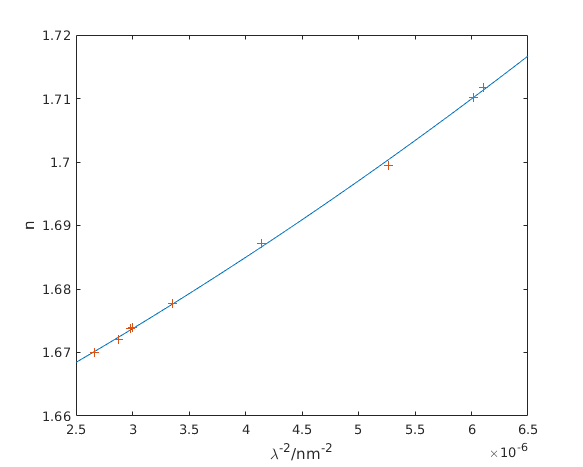
\includegraphics[scale=0.7]{figure.png}
	\caption{波长和折射率关系图线}
\end{figure}

	以$\lambda^{-2}$为横坐标, 用MATLAB拟合二次曲线, 图一为拟合出来的二次函数曲线. 各参数为
	
\begin{align*}
	n &= A + \frac{B}{\lambda^2} + \frac{C}{\lambda^4} \\
	A &= 1.6451 \\
	B &= 8.304 \times 10^3 nm^2 \\
	C &= 4.175 \times 10^8 nm^4
\end{align*}

\section{分析和讨论}

\subsection{误差来源分析}

	实验中每个数据都测量三次, 每次都测量两个游标读数, 所以随机误差很小. 实验中误差主要来自于以下方面:
	
\begin{enumerate}
	\item 测量色散曲线的时候, 两条黄线几乎无法区分, 难以观测到其差别. 角度上二者相差几乎只有1分. 
	\item 三棱镜顶角我没有测好, 以至于之后的实验中每次都会带来一些误差. 在掠入射法中, 三棱镜顶角的实验误差已经超过了其他因素带来的误差.
	\item 掠入射法测量的时候, 绿色十字一定要对准MN线的中央且左右转动表盘的时候绿色十字必须沿着MN线移动. 我在做实验的时候, 第一次没有调好绿色十字, 载物台不平行, 导致最后数据误差很大. 我重新完成了实验, 才测好了数据.
	\item 最小偏向角实验中, 最小偏向角的判定比较困难. 事实上没有很一般的判据的时候, 不但实验结果可能有偏差, 重复性都很差. 在数据中可以看到, 最小偏向角法的$\Delta \theta$的随机误差是要大于掠入射法的. 
\end{enumerate}

\subsection{为什么明暗分界线是一条弧线?}

	实验中我们用毛玻璃把钠灯的光变成一个面拓展光源, 这种方法虽然有效, 但是由于面拓展光源的辐射角度有一定范围, 所以最后观察到的现象是一个明暗过度的区域, 而不是一个真正的分界线. \\
	
	我们的光源到毛玻璃的路径上存在平行光管, 平行光管在毛玻璃上有一定投影, 加之我们的钠灯照射也不完全均匀(可能中间的光更加强烈一些), 这样就造成了这个明暗过渡的区域中间光强烈而上下边缘相对较暗, 最后看起来就像变成弧线一样.

\section{思考和感悟}

	这个实验是比较考验实验技巧的一个实验. 我一开始做实验的时候, 总是想着赶紧做完前面的实验去做拓展实验, 但是我做的太过匆忙, 导致我的载物台并没有完全调平, 最后掠入射法测折射率的实验数据非常糟糕. 而且我的顶角数据误差较大, 最后所有数据都会引用顶角数据, 以至于后面的实验误差也相对较大. \\
	
	我认识到, 实验不能着急! 要慢慢做, 每一步都要调好, 调妥当, 再进行下一步.
	
\end{CJK*}
\end{document}
